\vspace{-0.4\baselineskip}
\section{Approach}
\vspace{-0.4\baselineskip}
\label{sec:approach}

\begin{figure}
% \vspace{-0.5\baselineskip}
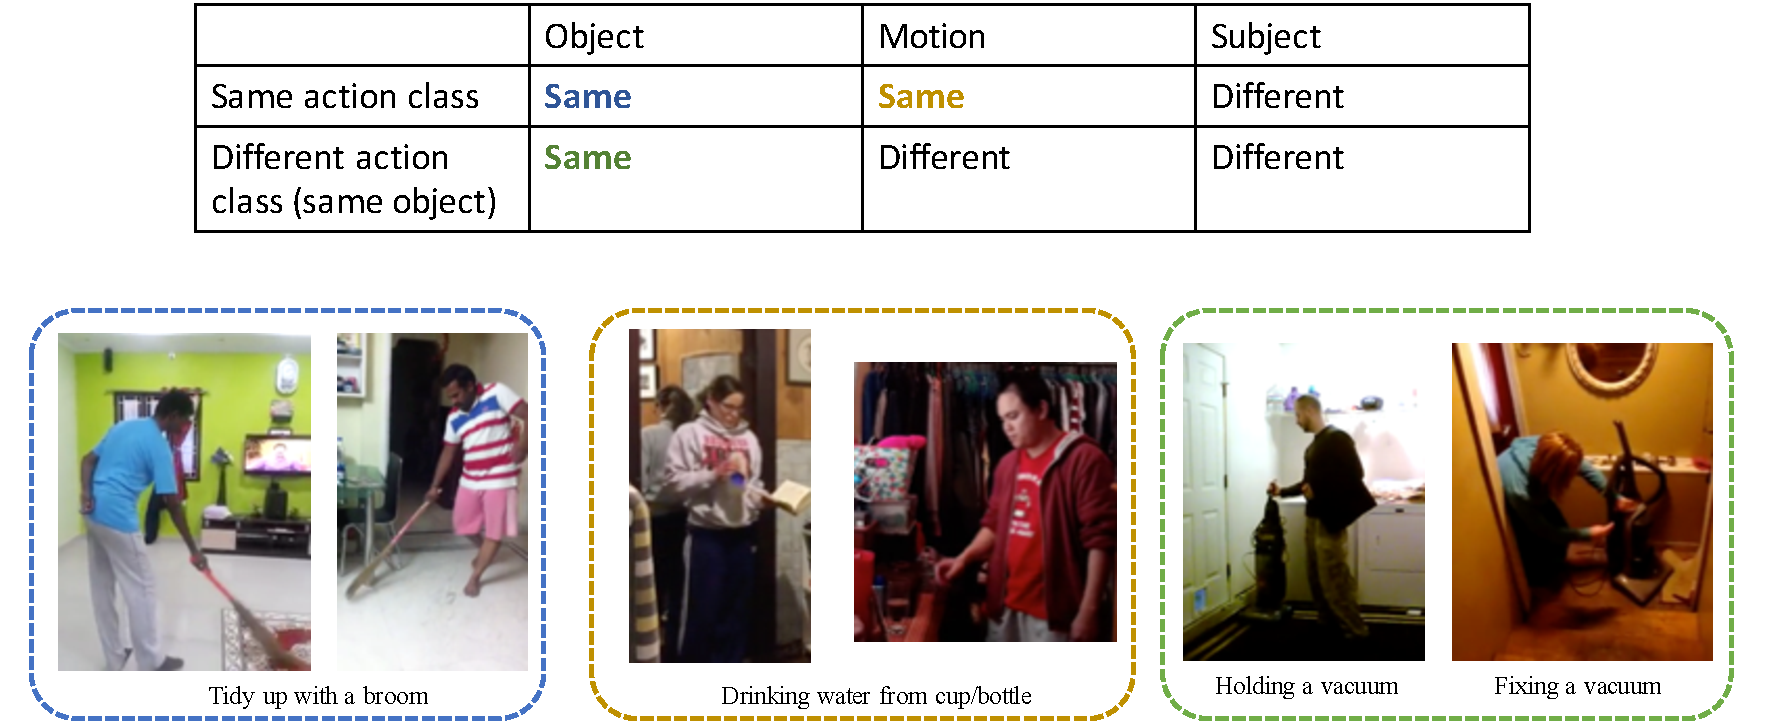
\includegraphics[width=0.5\textwidth]{figures/regularization_analysis.pdf}
% \caption{Visual comparison of depth and normal results between \protect\cite{zhou2017unsupervised} and ours. As the original depth ground truth map comes from sparse laser measurement, the interpolated depth map is shown for better visualization. As can be seen from the depth estimation, our results preserve the small/thin structures which have similar color to other foregrounds (green circles). From the normal comparison, our results predict the road normal direction better and have no artifact. The edges in normal map are also preserved better in our results (yello circles).}
\caption{Informations are listed in different axis. The consistencies that can be leveraged include colored cells.}
% \vspace{-0.8\baselineskip}
\label{fig:analysis}
\end{figure}

\begin{figure*}[ht!]
\centering
% \vspace{-0.5\baselineskip}
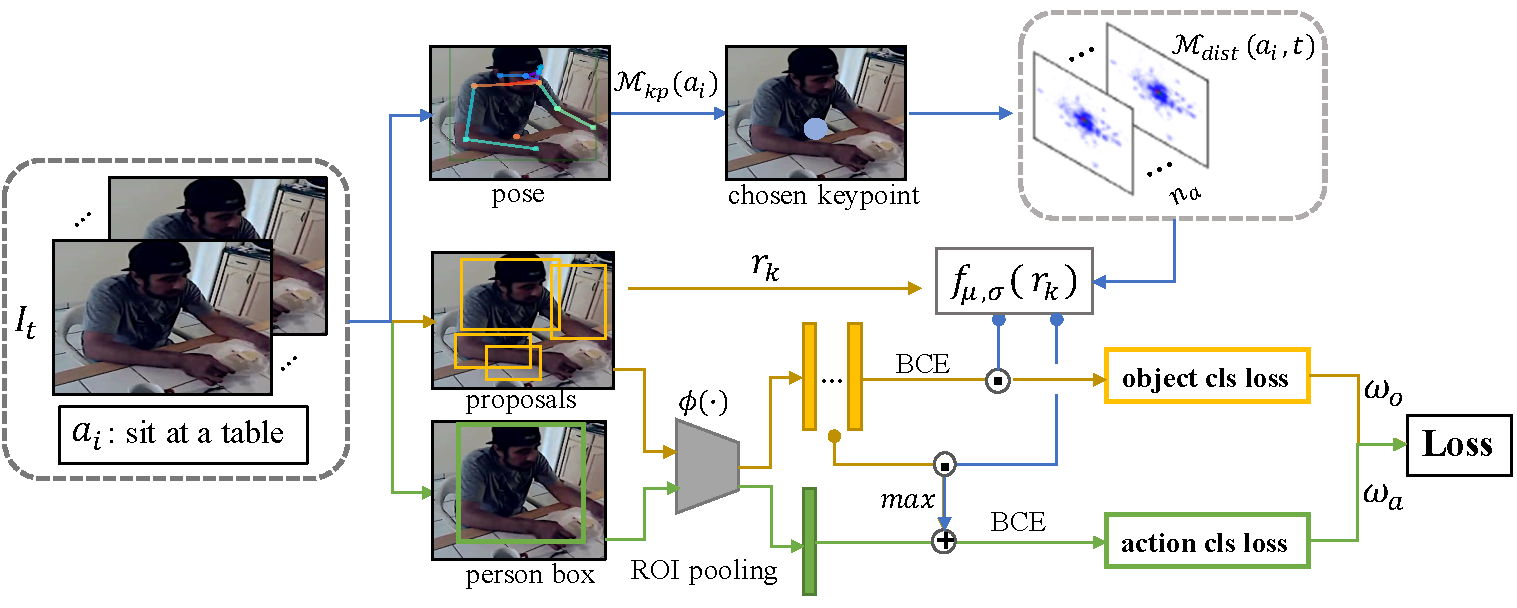
\includegraphics[width=0.8\textwidth]{figures/pipeline.pdf}
% \caption{Visual comparison of depth and normal results between \protect\cite{zhou2017unsupervised} and ours. As the original depth ground truth map comes from sparse laser measurement, the interpolated depth map is shown for better visualization. As can be seen from the depth estimation, our results preserve the small/thin structures which have similar color to other foregrounds (green circles). From the normal comparison, our results predict the road normal direction better and have no artifact. The edges in normal map are also preserved better in our results (yello circles).}
\caption{The object appearance is learned with a weakly supervised method by leveraging the three regularizations.}
% \vspace{-0.8\baselineskip}
\label{fig:pipeline}
\end{figure*}
% As discussed in \secref{sec:intro}, one major problem is that both~\cite{zhou2017unsupervised} and~\cite{yang2018aaai} have the regularization performed \wrt image gradient, which blocks nonlocal smoothness due to many false positives such as boundaries of shadows. 
In this section, we introduce the regularizaitons we apply to learn the object representation via supervision from action labels. To better show our analysis, the information that can be leveraged are listed in different axis in \figref{fig:analysis}. Basically, we propose to explore three constraints to help learning object appearance. The first one includes the appearance consistency of objects in the same action class (blue box in \figref{fig:analysis}). The other constrain comes from the motion consistency in the same action class. The motion of ``drinking water from cup/bottle'', including both subject and object motion, is similar across videos. Last but not least, the object appears similarly in videos of different action labels but involving same object category. In the actions ``holding vacuum'' and ``fixing vacuumm'' (green box in \figref{fig:analysis}), object appearances are consistent.



Based on the observations and regularizations above, we propose a weakly supervised pipeline for learning object detector. The proposed pipeline is shown in \figref{fig:pipeline}. The three regularzations are represented in this figure with corresponding colors as in \figref{fig:analysis}. Principlly, the appearance consistency in same action is leveraged by constructing object tubelets and the supervision comes from classification loss which favors the interacted objects (shown in blue stream). The object consistency across actions is modeled by incorporating the object tubelets from different action videos (but interacting with the same object). The motion of subject/object should be distinguishable across different actions, thus the motion consistency is leveraged by the third stream which classify the video based on motion features from subject and object. 



